%#% extstart input preamble.tex
%
% memman.tex  Memoir class user manual (Part II only)  last updated 2009/09/07
%             Author: Peter Wilson
%             Copyright 2001, 2002, 2003, 2004, 2008, 2009 Peter R. wilson
%
%   This work has the LPPL maintenance status "maintained".
%   Maintainer: Lars Madsen (daleif at math dot au dot dk)
%
%\listfiles
\documentclass[10pt,extrafontsizes]{memoir}
\usepackage{comment}
\usepackage[table,xcdraw, dvipsnames]{xcolor}
%\usepackage{quotchap}
%\usepackage[Bjornstrup]{fncychap}
\setlength{\parindent}{0cm}
\usepackage{caption}
\usepackage{subcaption}
\usepackage{adjustbox}
\usepackage{lscape}
\usepackage{geometry}
\usepackage{psvectorian}
%\usepackage[natbibapa]{apalike}
\usepackage{natbib} 
\usepackage{arydshln}
%\usepackage{hyperref}

%%%%%%%%%%%%%%%%%%%%%%%%
\usepackage[T1]{fontenc}
\usepackage{kpfonts}
\setSingleSpace{1.1}
\SingleSpacing
\usepackage{xcolor, calc, blindtext}
\definecolor{chaptercolor}{gray}{0.8}
% helper macros
\newcommand\numlifter[1]{\raisebox{-2cm}[0pt][0pt]{\smash{#1}}}
\newcommand\numindent{\kern37pt}
\newlength\chaptertitleboxheight
\makechapterstyle{hansen}{
  \renewcommand\printchaptername{\raggedleft}
  \renewcommand\printchapternum{%
    \begingroup%
    \leavevmode%
    \chapnumfont%
    \strut%
    \numlifter{\thechapter}%
    \numindent%
\endgroup%
}
  \renewcommand*{\printchapternonum}{%
    \vphantom{\begingroup%
      \leavevmode%
      \chapnumfont%
      \numlifter{\vphantom{9}}%
      \numindent%
      \endgroup}
    \afterchapternum}
  \setlength\midchapskip{0pt}
  \setlength\beforechapskip{0.5\baselineskip}
  \setlength{\afterchapskip}{3\baselineskip}
  \renewcommand\chapnumfont{%
    \fontsize{4cm}{0cm}%
    \bfseries%
    \sffamily%
    \color{chaptercolor}%
  }
  \renewcommand\chaptitlefont{%
    \normalfont%
    \huge%
    \bfseries%
    \raggedleft%
  }%
  \settototalheight\chaptertitleboxheight{%
    \parbox{\textwidth}{\chaptitlefont \strut bg\\bg\strut}}
  \renewcommand\printchaptertitle[1]{%
    \parbox[t][\chaptertitleboxheight][t]{\textwidth}{%
      %\microtypesetup{protrusion=false}% add this if you use microtype
      \chaptitlefont\strut ##1\strut}%
}}
\chapterstyle{hansen}
\aliaspagestyle{chapter}{empty} % just to save some space

%%%%%%%%%%%%%%%%%%%%%%%%

%%%%%%%%%%%%%%%%%%%

\hfuzz=5pt

%\setlength\overfullrule{5pt}


% For (non-printing) notes  \PWnote{date}{text}
\newcommand{\PWnote}[2]{} 
\PWnote{2009/04/29}{Added fonttable to the used packages}
\PWnote{2009/08/19}{Made Part I a separate doc (memdesign.tex).}

% same
\newcommand{\LMnote}[2]{} 


\usepackage{memsty}
%%%%%%%%%%%%%%%%%%%%%%%%%%%%
\usepackage{titlepages}  % code of the example titlepages
\usepackage{memlays}     % extra layout diagrams
\usepackage{dpfloat}     % floats on facing pages
\usepackage{fonttable}[2009/04/01]   % font tables
%%%%\usepackage{xr-hyper} \externaldocument{memdesign} Doesn't work, 
%%%%                      Idea won't work in general for memman/memdesign
%%%%                      as at display time, who knows where everything
%%%%                      will be located on the individual's computer.
%%%%%%%%%%%%%%%%%%%%%%%%%%%%

%%%% Change section heading styles
%%%\memmansecheads

%%%% Use the built-in division styling
\headstyles{memman}

%%% ToC down to subsections
\settocdepth{subsubsection}
%%% Numbering down to subsections as well
\setsecnumdepth{subsubsection}

%%%% extra index for first lines
%\makeindex[lines]


% this 'if' is used to determine whether we are compiling the memoir
% master in the subversion repository, or the public memman.tex
\newif\ifMASTER
\MASTERfalse
%\MASTERtrue

\ifMASTER

% add patch to fink, such that \AtEndFile still work
\makeatletter
\AtEndFile{fink.sty}{
  \typeout{patching fink} 
  \renewcommand{\InputIfFileExists}[2]{%
    \IfFileExists{##1}%
    {##2\@addtofilelist{##1}%
      \m@matbeginf{##1}%
      \fink@prepare{##1}%
      %\@@input \@filef@und
      \expandafter\fink@input%
      \expandafter\fink@restore\expandafter{\finkpath}%
     \m@matendf{##1}%
     \killm@matf{##1}}%
 }
}
\makeatother
% private package, not in circulation
% enables us to gather svn information on a single file basis
%\usepackage[filehooks]{svn-multi-private}
% use the current version
\usepackage[filehooks]{svn-multi}


% \svnidlong
% {}
% {$LastChangedDate: 2020-03-25 19:00:55 +0100 (Wed, 25 Mar 2020) $}
% {$LastChangedRevision: 686 $}
% {$LastChangedBy: daleif@math.au.dk $}



\makeatletter
\newcommand\addRevisionData{%
  \begin{picture}(0,0)%
    \put(0,-20){%
      \tiny%
      \expandafter\@ifmtarg\expandafter{\svnfiledate}{}{%
        \textit{\textcolor{darkgray}{Chapter last updated \svnfileyear/\svnfilemonth/\svnfileday
         \enspace (revision \svnfilerev)}}
     }%
    }%
  \end{picture}%
}
\makeatother

% we add this to the first page of each chapter

\makepagestyle{chapter}
\makeoddfoot{chapter}{\addRevisionData}{\thepage}{}
\makeevenfoot{chapter}{\addRevisionData}{\thepage}{}

\else
% disable svn info collecting
\newcommand\svnidlong[4]{}
\fi

%% end preamble
%%%%%%%%%%%%%%%%%%%%%%%%%%%%%%%%%%%%%%%%%%%%%%%%%%%%%%%
%#% extend


%\hfuzz=10pt

\usepackage[draft]{fixme}
\fxsetup{
  multiuser,
  marginface=\normalfont\tiny,
  innerlayout=noinline,
  layout=marginnote,
}
\usepackage{tikz,ragged2e}
\makeatletter
% extra feature, vadj=length kan flytte på fxnotes hvis de overlapper
\@fxdefinekey{layout}{vadj}{\def\marginnotevadjust{#1}}

% endnu mere ekstra feature, kræver tikz og calc tikz lib

\renewcommand*\FXLayoutMarginNote[3]{%
  \tikz[overlay,remember picture]\coordinate (A) at (0,0);%
  \marginnote[%
    \RaggedLeft%
    \rlap{\tikz[overlay,remember picture]\coordinate(C) at (0,0);}%
    \@fxuseface{margin}%
    \@fxtextstd{#1}{#2}{#3}%
    {\tikz[overlay,remember picture,ultra thin,cyan]\draw(A) -| ++(0,-2pt) -|(C);}%
  ]{%
    \RaggedRight%
    \tikz[overlay,remember picture]\coordinate(B) at (0,0);%
    \@fxuseface{margin}%
    \@fxtextstd{#1}{#2}{#3}%
    \tikz[overlay,remember picture,ultra thin,cyan]\draw(A) -| ++(0,-2pt) -|(B);%
  }%
}
\makeatother



\begin{document}


%#% extstart input intro.tex

% Coarse-to-fine Curriculum Learning in LiDAR semantic segmentation by contrasting visual representations.



%\tightlists
\firmlists
\midsloppy
\raggedbottom
\chapterstyle{hansen}
%%%%%%%%%%%%%%%%%%%%%%%%%%%%%%%%%%%%%%%%%%%%%%%%%%%%


\ProvidesFile{memnoidxnum}[2009/04/30  some index entries for memman]
\newcommand*{\idxat}{\index{@?\texttt{@}|noidxnum}} \idxat
%%\index{@?\texttt{@}|noidxnum}
\index{argument|noidxnum}
%%\index{array|noidxnum}
\index{cardinal|noidxnum}
\index{centering|noidxnum}
%%\index{chapterstyle|noidxnum}
%%\index{counter|noidxnum}
\index{default|noidxnum}
\index{division|noidxnum}
\index{division!sectional|seealso{subhead}}
\index{double column|noidxnum}
\index{endnote!mark|seealso{reference mark}}
\index{environment|noidxnum}
\index{error message|noidxnum}
\index{figures|noidxnum}
%%\index{file|noidxnum}
\index{font characteristic|noidxnum}
\index{footnote!mark|seealso{reference mark}}
\index{footnotes|noidxnum}
\index{frame|noidxnum}
\index{framed|noidxnum}
\index{full stop|seealso{period}}
\index{hanging|noidxnum}
\index{headstyles|noidxnum}
%%\index{horizontal|noidxnum}
\index{Hurenkinder|see{widow}}
\index{interlinear space|see{leading}}
\index{keyword|noidxnum}
%%\index{label|noidxnum}
\index{LaTeX?\ltx|noidxnum}
%%\index{length|noidxnum}
\index{line|noidxnum}
\index{line too long|see{overfull lines}}
\index{lining|noidxnum}
%%\index{list|noidxnum}
\index{lowercase|noidxnum}
\index{MakeIndex?\Pmakeindex|noidxnum}
\index{margin!spine|seealso{inner}}
\index{margin!inner|seealso{spine}}
\index{margin!foredge?\foredge|seealso{outer}}
\index{margin!outer|seealso{\foredge}}
\index{margin!upper|seealso{top}}
\index{margin!top|seealso{upper}}
\index{math|noidxnum}
%%\index{memoir class|noidxnum}
\index{minipage|noidxnum}
\index{name|noidxnum}
\index{named|noidxnum}
\index{new|noidxnum}
%%\index{number|noidxnum}
\index{numeric|noidxnum}
\index{old-style|noidxnum}
\index{option|noidxnum}
\index{ordinal|noidxnum}
\index{outline|noidxnum}
\index{package|noidxnum}
\index{page break|noidxnum}
%%\index{pagestyle|noidxnum}
\index{paragraph break|noidxnum}
\index{period|seealso{full stop}}
\index{poem|noidxnum}
\index{program|noidxnum}
\index{ranging|noidxnum}
\index{reference|noidxnum}
\index{reference mark|seealso{endnote mark, footnote mark}}
\index{representation|noidxnum}
\index{rule|noidxnum}
\index{ruled|noidxnum}
%%\index{section|noidxnum}
\index{Schusterjungen|see{orphan}}
\index{section|seealso{subhead}}
\index{sectional division|seealso{subhead}}
\index{single column|noidxnum}
\index{size|noidxnum}
\index{space|noidxnum}
\index{space!double|see(double spacing)}
\index{space!between lines|see{leading}}
\index{stanza|noidxnum}
%%\index{subfloat|noidxnum}
\index{TeX?\tx|noidxnum}
\index{text|noidxnum}
\index{titling|noidxnum}
\index{trim|noidxnum}
%%\index{type size|noidxnum}
\index{vertical|noidxnum}
\index{warning|noidxnum}
\index{write|noidxnum}
%%\index{XeTeX?\xetx|noidxnum}

%%%%%%%% Deleted the font indexing (now done as typefaces) 2009/04/30

\begin{comment}
\index{table of contents|see{ToC}}
\index{list!of figures|see{LoF}}
\index{figure!list of|see{LoF}}
\index{list!of tables|see{LoT}}
\index{table!list of|see{LoT}}
\index{marginal note|see{marginalia}}
\index{footnote!in title|see{thanks}}
\index{illustration|seealso{float, figure}}
\index{figure|seealso{float}}
\index{table|seealso{float}}
\index{chapter!style|see{chapterstyle}}
\index{chapter!heading|see{heading}}
\index{page!style|see{pagestyle}}
\index{part!heading|see{heading}}
\end{comment}

\begin{comment}

%%%% deleted the \nocites
%
\index{anonymous division|see{division}}
\index{array|seealso{tabular}}
%
\index{Berne Convention|see{copyright}}
\index{blank page|see{page}}
\index{Buenes Aires Convention|see{copyright}}
\index{box!rule|seealso{rule}}
%
\index{chapter|seealso{division}}
\index{chapter!style|see{chapterstyle}}
\index{command|seealso{declaration, macro}}
\index{comptexttex?\texttt{comp.text.tex} newsgroup|see{\ctt}}
\index{Comprehensive TeX Archive Network?\cTeXan|see{\ctan}}
\index{contents list|see{ToC}}
\index{counter representation!Alph tt?\texttt{Alph}|see{\texttt{Alph}}}
\index{counter representation!alph tt?\texttt{alph}|see{\texttt{alph}}}
\index{counter representation!arabic tt?\texttt{arabic}|see{\texttt{arabic}}}
\index{counter representation!Roman tt?\texttt{Roman}|see{\texttt{Roman}}}
\index{counter representation!roman tt?\texttt{roman}|see{\texttt{roman}}}
\index{counter representation!fnsymbol tt?\texttt{fnsymbol}|see{\texttt{fnsymbol}}}
\index{cross reference|seealso{reference}}
%
\index{descriptive list|see{list}}
\index{display math|see{math}}
\index{display mode|see{display}}
\index{division|seealso{heading}}
%
\index{electronic book|see{ebook}}
\index{enumerated list|see{list}}
%
\index{figure!list of|see{LoF}}
\index{figure|seealso{float}}
\index{float!numbered captioning|see{caption}}
\index{float!unnumbered captioning|see{legend}}
\index{font characteristic!weight|see{series}}
%
\index{file|seealso{stream}}
\index{footnote!in title|see{thanks}}
\index{fragile command|seealso{protect}}
\index{free tabular|seealso{tabular}}
%
\index{header|seealso{running header}}
\index{heading|seealso{division}}
%
\index{illustration|seealso{float, figure}}
\index{inline math|see{math}}
\index{International Standard Book Number|see{ISBN}}
\index{itemized list|see{list}}
%
\index{label|seealso{reference}}
\index{left-to-right|see{LR}}
\index{list!new list of|see{list of, new}}
\index{list!of contents|see{ToC}}
\index{list!of figures|see{LoF}}
\index{list!of tables|see{LoT}}
\index{list of!contents|see{ToC}}
\index{list of!figures|see{LoF}}
\index{list of!tables|see{LoT}}
\index{LoF|seealso{ToC}}
\index{LoT|seealso{ToC}}
\index{log-like function|see{function}}
%
\index{macro|seealso{command}}
\index{margin note|seealso{marginalia}}
\index{marginalia|seealso{marginal note, side note, sidebar}}
%
\index{named division|see{division}}
%
\index{page!of floats|see{float, page}}
\index{page!start new|see{start new page}}
\index{page!style|see{pagestyle}}
\index{paragraph|seealso{division}}
\index{part|seealso{division}}
\index{picture object!Bezier curve|see{Bezier curve}}
\index{picture object!circle|see{circle}}
\index{picture object!line|see{line}}
\index{picture object!oval|see{box, rounded}}
\index{picture object!vector|see{vector}}
\index{poem|see{verse}}
\index{poetry|see{verse}}
\index{print run|see{impression}}
\index{protect|seealso{fragile command}}
%
\index{recto|seealso{odd page}}
\index{reference|seealso{label}}
\index{river|see{white space}}
\index{rivulet|see{white space}}
\index{running footer|see{footer}}
\index{running header|seealso{header}}
%
\index{section|seealso{division}}
\index{side note|seealso{marginalia}}
\index{sidebar|seealso{marginalia}}
\index{stanza|seealso{verse}}
\index{stanza!line number|see{line number}}
\index{subparagraph|seealso{division}}
\index{subsection|seealso{division}}
\index{subsubsection|seealso{division}}
%
\index{table of contents|see{ToC}}
\index{table!list of|see{LoT}}
\index{table|seealso{float}}
\index{tabular|seealso{array}}
\index{tabular!free|see{free tabular}}
\index{tabulation|see{tabular}}\
\index{TeX Users Group?\TeXUG|see{\tug}}
\index{textblock|see{typeblock}}
%
\index{Universal Copyright Convention|see{copyright}}
%
\index{verbatim!line number|see{line number}}
\index{verse|seealso{stanza}}
\index{verse!title|see{poem title}}
\index{verse!line number|see{line number}}
\index{verso|seealso{even page}}
\index{visual markup|see{visual design}}
%
\index{x coordinate|see{coordinate}}
%
\index{y coordinate|see{coordinate}}
%
%


\end{comment}

\endinput



%In the middle if you want to change the margins use
\newgeometry{left=0.7in,right=0.5in,top=1in,bottom=1in}
\clearpage
\pagestyle{empty}
\newpage

%%%%%%%%%%%%%%%%%%%%%%%%%%%%%%%%%%%%%%%%%%%%%%%%%%%%
%%%%		   PERSONALIZED TITLEPAGE   	    %%%%

% author: Elena Camuffo Copyright 2021
% insert here the data for the titlepage

\definecolor{M2}{HTML}{9B0014}
\definecolor{SchoolColor}{rgb}{0.71, 0, 0.106} %Unipd color

\newcommand{\UnivName}{University of Padova}
\newcommand{\UnivPlace}{Padova}
\newcommand{\DeptName}{Information Engineering}

\newcommand{\DegreeName}{Master Degree in ICT for internet and multimedia}
\newcommand{\ThesisTitle}{Curriculum and Contrastive Learning\\in LiDAR Semantic Segmentation}

\newcommand{\SupName}{Simone}
\newcommand{\SupSurname}{Milani}

%comment these lines if there are no supervisors
\newcommand{\CosupName}{Umberto}
\newcommand{\CosupSurname}{Michieli}

\newcommand{\AuthName}{Elena}
\newcommand{\AuthSurname}{Camuffo}

\newcommand{\AcademicYear}{2020-2021}
\newcommand{\GraduationDay}{September 6, 2021}
%%%%

% print the titlepage
\mytitle

%%%%%%%%%%%%%%%%%%%%%%%%%%%%%%%%%%%%%%%%%%%%%%%%%%%%

\vspace{2\baselineskip}
\cleardoublepage

%%%%%%%%%%%%%%%%% DEDICATION %%%%%%%%%%%%%%%%%%%%%%%
\clearpage
\begin{center}
    \thispagestyle{empty}
    \vspace*{\fill}
    \psvectorian[scale=0.5]{188}
    \vspace{0.5cm}\\
    \textsc{Dedication.}
        \vspace*{\fill}
\end{center}
\cleardoublepage
%\restoregeometry

%%%%%%%%%%%%%%%%%%%  QUOTE  %%%%%%%%%%%%%%%%%%%%%%%%
\clearpage
\begin{center}
    \thispagestyle{empty}
    \vspace*{\fill}
    %\psvectorian[scale=0.5]{183}\vspace{0.5cm}\\
\emph{"Simplicity is the end result of long, hard work, not the starting point. "} \\
\vspace{0.2cm}
- Frederick Maitland -
    \vspace*{\fill}
\end{center}
\cleardoublepage
\restoregeometry


% Abstract: Remove indents around abstract text
\setlength{\absleftindent}{0pt}
\setlength{\absrightindent}{0pt}
% Change font size to conform with the rest of the document text
\renewcommand{\abstracttextfont}{\normalsize}
\abstractintoc % Include "Abstract" in ToC

\chapter*{Abstract}\label{ch:abstract}
Recent advances in technologies such as autonomous driving and robotics have highlighted the growing need for precise environmental perception. LiDAR Semantic Segmentation has recently attracted the attention of industrial and academic research due to its ability to accomplish fine-grained scene understanding and act directly on raw content provided by sensors. The task has been approached in a variety of ways, so far. RandLA-Net architecture has been selected for this work as it represents a powerful and lightweight solution to deal with large-scale data. The goal of developing solutions that aim at optimizing the learning process rather than focusing on the architecture has been considered, showing how different learning techniques can be used to improve the performance of the model. The methods include Curriculum Learning and Contrastive Learning, which aim at having a better separation between different classes, providing a better understanding of the scene content. Coarse-to-Fine strategies have been developed as well as regularization methods in order to take into account a hierarchical organization of the classes. The results we obtained outperform the state of the art, achieving an improvement of $1.5\%$ in terms of mIoU with different methods. They proved their efficiency by providing a better balance of classes and a faster convergence to optimal performance.
\cleardoublepage
\chapter*{Sommario}\label{ch:sommario}
Lo sviluppo recente di tecnologie come la guida autonoma e la robotica hanno evidenziato la crescente necessit� di una pi� accurata percezione dell'ambiente da parte dei dispositivi. La segmentazione semantica LiDAR ha recentemente attirato l'attenzione della ricerca industriale e accademica, grazie alla sua capacit� di comprendere in modo preciso il contenuto della scena percepita e agire direttamente sui dati grezzi forniti dai sensori. A tale scopo sono state proposte diverse soluzioni algoritmiche. RandLA-Net � stata scelta come architettura per questo lavoro, in quanto rappresenta una soluzione potente e leggera per gestire dati su larga scala. L'obiettivo della tesi � sviluppare una procedura per ottimizzare il processo di apprendimento  di RandLA-Net invece di andare a modificare la struttura della rete, mostrando come diverse tecniche di apprendimento possano migliorare le prestazioni a parit� di modello, dataset e risorse di calcolo. I metodi includono l'apprendimento curriculare (Curriculum Learning) e l'apprendimento contrastivo (Constrastive Learning), i quali mirano ad ottenere una migliore separazione tra le diverse classi, basandosi su un raggruppamento gerarchico a posteriori e fornendo una migliore comprensione del contenuto della scena. Strategie Coarse-to-Fine e metodi di regolarizzazione sono stati impiegati per tenere conto di un'organizzazione gerarchica delle classi. I risultati dei nostri metodi superano lo stato dell'arte, ottenendo un miglioramento di $1.5\%$ in termini di mIoU con diversi metodi. Hanno dimostrato la loro efficienza, fornendo un migliore equilibrio delle classi e una convergenza pi� rapida verso le prestazioni ottimali.
\cleardoublepage

% ToC, etc
%\pagenumbering{roman}
\pagestyle{Ruled}

%%%%%%%%%%%%%%% TABLES OF CONTENT %%%%%%%%%%%%%%%%%%
%\setupshorttoc
\tableofcontents
\clearforchapter
\setupparasubsecs
\setupmaintoc

\setlength{\unitlength}{1pt}
\clearpage
\listoffigures
\clearpage
\listoftables
\cleardoublepage
%\listofegresults
%\clearpage
%\nomenclature

%#% extend
%#% extstart include preface.tex
%\chapter{Foreword}

\svnidlong
{$Ignore: $}
{$LastChangedDate: 2014-11-05 16:28:11 +0100 (Wed, 05 Nov 2014) $}
{$LastChangedRevision: 501 $}
{$LastChangedBy: daleif $}

%%%%%%%%%%%%%%  CHAPTERS  %%%%%%%%%%%%%%%%%%%
\chapter{Introduction}\label{ch:intro}

\textit{In this chapter a brief overview of the problem and the contribution of our work  is given.}

\par\fancybreak{$***$}\par
\vspace{0.35cm} 

Lorem ipsum dolor sit amet, consectetur adipisci elit, sed eiusmod tempor incidunt ut labore et dolore magna aliqua. Ut enim ad minim veniam, quis nostrum exercitationem ullam corporis suscipit laboriosam, nisi ut aliquid ex ea commodi consequatur. Quis aute iure reprehenderit in voluptate velit esse cillum dolore eu fugiat nulla pariatur. Excepteur sint obcaecat cupiditat non proident, sunt in culpa qui officia deserunt mollit anim id est laborum.

\begin{figure}[h]
 \centering
     \begin{subfigure}[b]{0.3\textwidth}
         \centering
         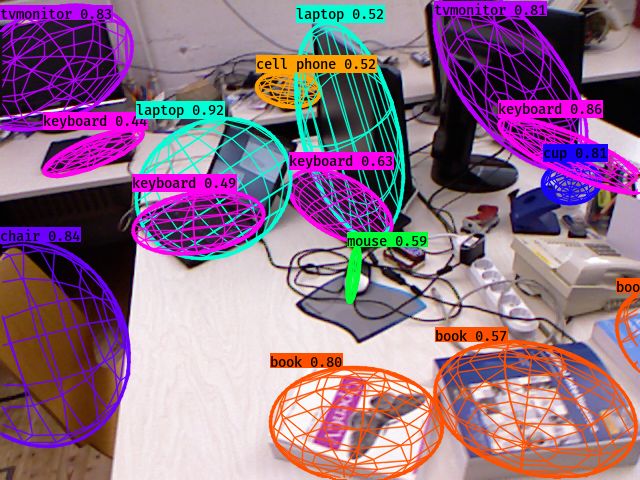
\includegraphics[width=\textwidth]{Figures/Introduction/app1.png}
         \caption{Robotics.}
         \label{fig:app1}
     \end{subfigure}
     \hfill
     \begin{subfigure}[b]{0.35\textwidth}
         \centering
         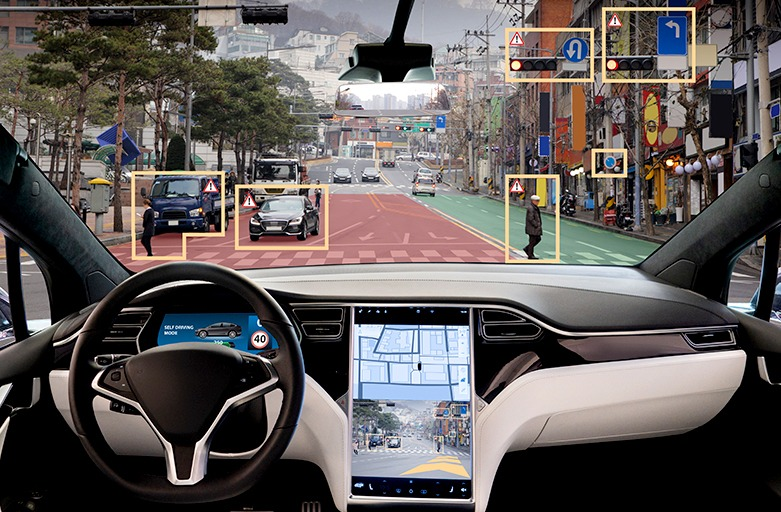
\includegraphics[width=\textwidth]{Figures/Introduction/app2.jpg}
         \caption{Self-driving cars.}
         \label{fig:app2}
     \end{subfigure}
     \hfill
     \begin{subfigure}[b]{0.3\textwidth}
         \centering
         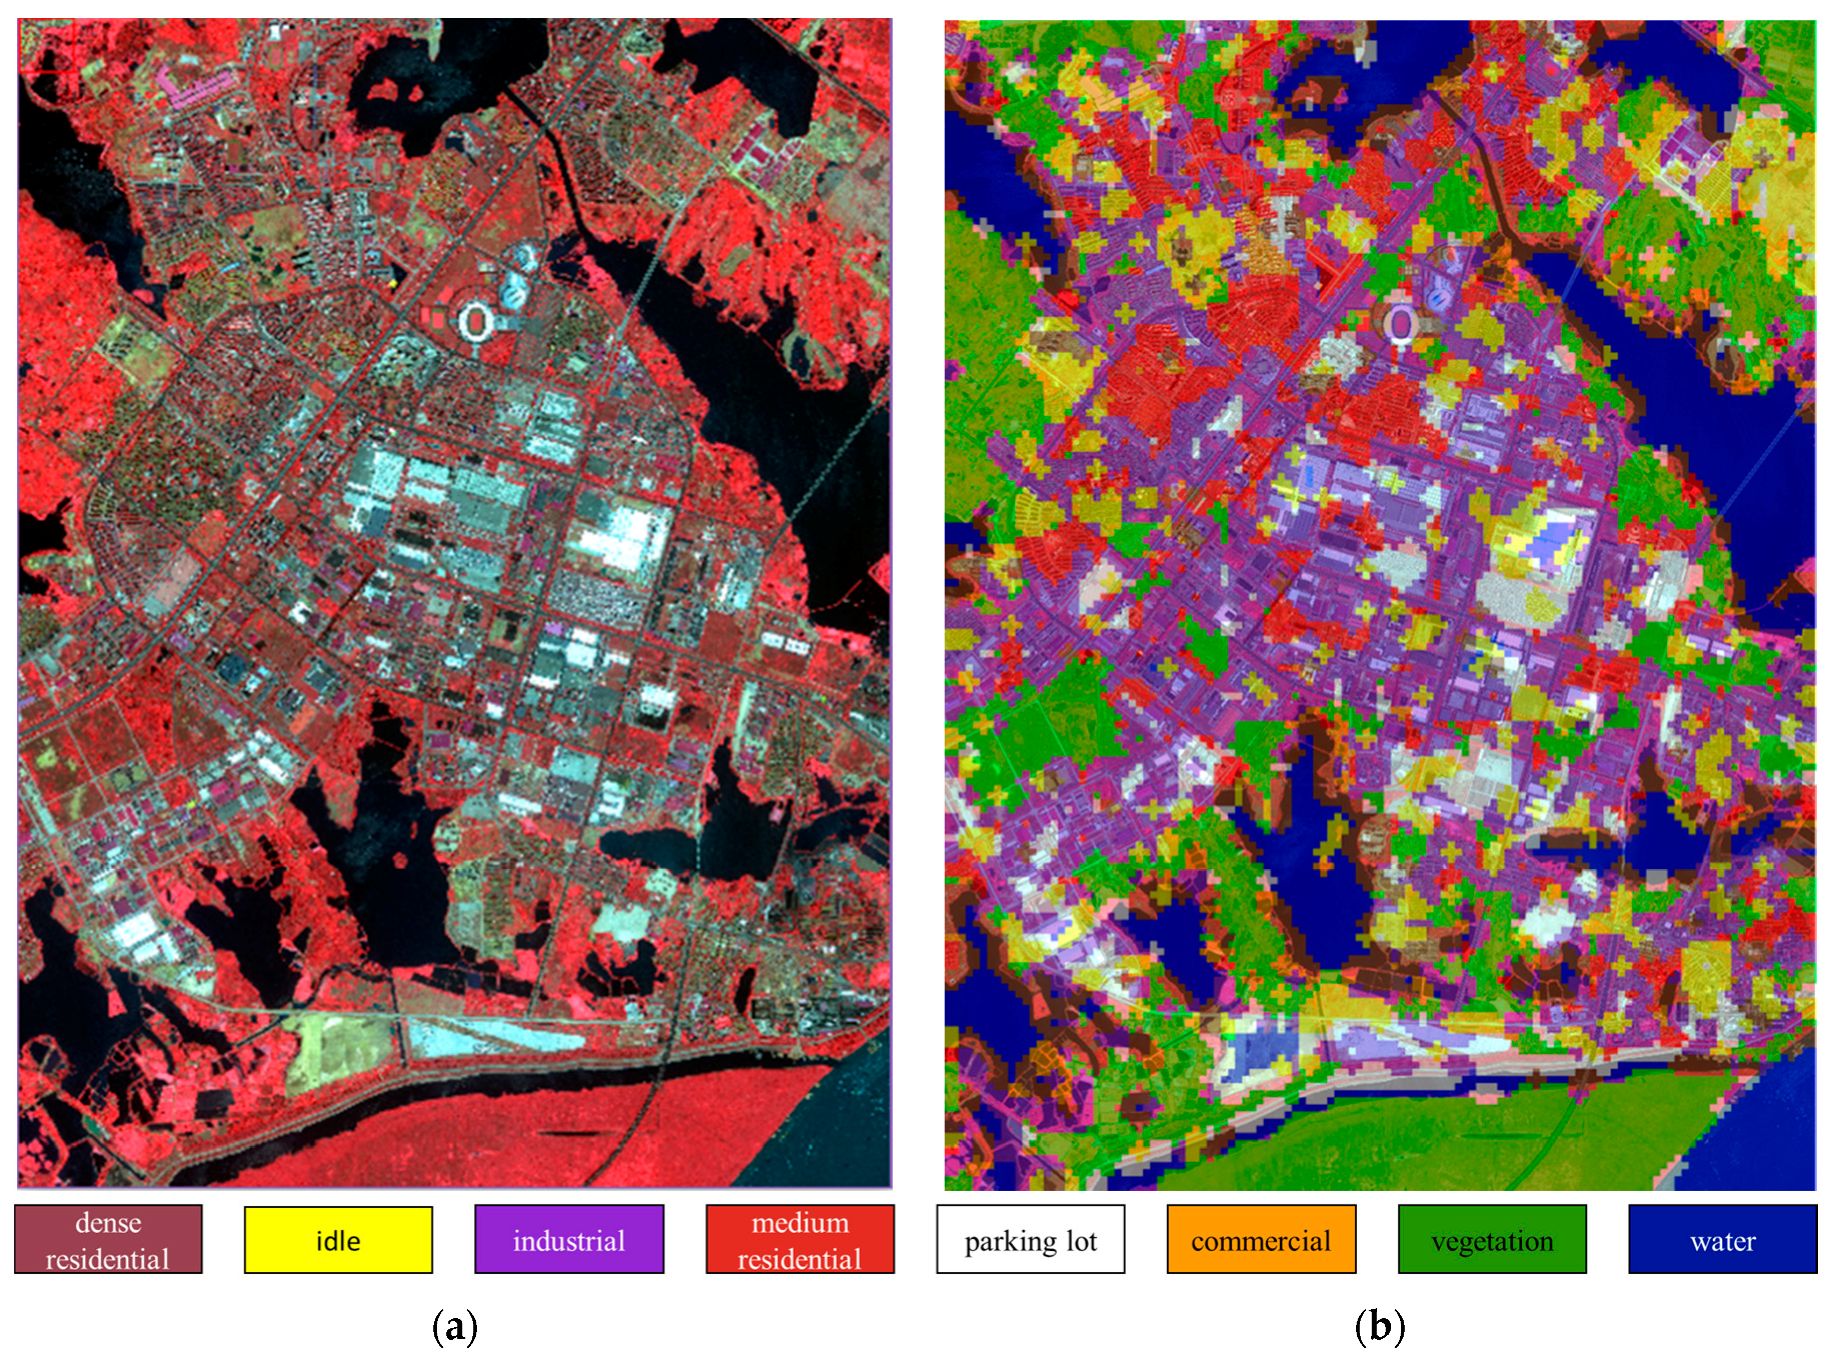
\includegraphics[width=\textwidth]{Figures/Introduction/app3.png}
         \caption{Remote sensing.}
         \label{fig:app3}
     \end{subfigure}
\caption{Examples of three figures side by side.}        
\label{fig:applications}
\end{figure}
\chapter{Theoretical Background}\label{ch:bg}
\textit{In this chapter the theoretical background of the overall work is presented, giving insights on the methods adoped.}
\vspace{0.25cm}
\par\fancybreak{$***$}\par
\vspace{0.35cm}

Lorem ipsum dolor sit amet, consectetur adipisci elit, sed eiusmod tempor incidunt ut labore et dolore magna aliqua. Ut enim ad minim veniam, quis nostrum exercitationem ullam corporis suscipit laboriosam, nisi ut aliquid ex ea commodi consequatur. Quis aute iure reprehenderit in voluptate velit esse cillum dolore eu fugiat nulla pariatur. Excepteur sint obcaecat cupiditat non proident, sunt in culpa qui officia deserunt mollit anim id est laborum \cite{hu2020randlanet}.

In mathematical terms:
\begin{equation}
\mathcal{L}_{CE} = -\sum_{i=1}^{N}p_i \log p_i
\end{equation}
\chapter{Results}\label{ch:results}
\textit{In this chapter the results of the simulations led are presented.}
\vspace{0.25cm}
\par\fancybreak{$***$}\par
\vspace{0.35cm}

Lorem ipsum dolor sit amet, consectetur adipisci elit, sed eiusmod tempor incidunt ut labore et dolore magna aliqua. Ut enim ad minim veniam, quis nostrum exercitationem ullam corporis suscipit laboriosam, nisi ut aliquid ex ea commodi consequatur. Quis aute iure reprehenderit in voluptate velit esse cillum dolore eu fugiat nulla pariatur. Excepteur sint obcaecat cupiditat non proident, sunt in culpa qui officia deserunt mollit anim id est laborum.

\begin{table}[h]
\centering
\setlength{\tabcolsep}{2pt}
\resizebox{\textwidth}{!}{%
\begin{tabular}{r|c|ccccccccccccccccccc}
Trial   name & \rotatebox{90}{mIoU} & \rotatebox{90}{car}  & \rotatebox{90}{bicycle} & \rotatebox{90}{motorcycle} & \rotatebox{90}{truck} & \rotatebox{90}{other-vehicle} & \rotatebox{90}{person} & \rotatebox{90}{bicyclist} & \rotatebox{90}{motorcyclist} & \rotatebox{90}{road} & \rotatebox{90}{parking} & \rotatebox{90}{sidewalk} & \rotatebox{90}{other-ground} & \rotatebox{90}{building} & \rotatebox{90}{fence} & \rotatebox{90}{vegetation} & \rotatebox{90}{trunk} & \rotatebox{90}{terrain} & \rotatebox{90}{pole} & \rotatebox{90}{traffic-sign} \\
\hline
Original          & 52.91 & 92.94 & 12.67   & 28.43      & 70.02 & 35.62         & 52.31  & 69.03     & 0.00         & 91.15 & 37.06   & 75.96    & 1.45         & 87.62    & 43.68 & 84.95      & 60.23 & 73.67   & 51.56 & 36.93        \\
fairness $\gamma=10$ + C2F  & 53.00    & 93.3 0 & 11.31   & 29.96      & 76.27 & 40.53         & 49.24  & 55.34     & 0.00            & 91.49 & 39.06   & 76.75    & 1.59         & 87.63    & 45.36 & 85.64      & 60.30  & 73.90    & 52.59 & 36.80         \\
hierarchy $\gamma=0.01$ + fairness $\gamma=10$  & 53.87 & 93.23 & 16.33   & 32.23      & 66.55 & 41.18         & 52.92  & 67.67     & 0.00            & 91.79 & 39.91   & 76.65    & 0.45         & 87.78    & 43.96 & 85.41      & 62.13 & 73.26   & 52.95 & 39.09        \\
hierarchy $\gamma=0.01$ + C2F    & 52.95 & 93.18 & 15.51   & 27.69      & 72.37 & 40.62         & 44.61  & 67.77     & 0.00            & 91.54 & 39.36   & 76.83    & 0.68         & 87.78    & 42.24 & 84.99      & 59.62 & 75.51   & 51.16 & 34.63  \\
hierarchy   $\gamma=0.05$ + fairness $\gamma=10$       & 53.99 & 92.83 & 17.72 & 30.83 & 73.59 & 38.74 & 49.96 & 69.87 & 0.00 & 91.64 & 42.39 & 76.92 & 3.29 & 87.33 & 44.12 & 85.15 & 58.52 & 73.89 & 51.15 & 37.91 \\
hierarchy   $\gamma=0.01$ + fairness $\gamma=10$ + C2F & 54.12 & 93.12 & 15.42 & 34.01 & 63.76 & 40.66 & 53.83 & 66.63 & 0.00 & 91.54 & 40.78 & 77.11 & 1.34 & 89.16 & 48.93 & 85.47 & 61.58 & 73.45 & 52.48 & 39.06 \\
hierarchy   $\gamma=0.05$ + fairness $\gamma=10$ + C2F & \textbf{54.34} & 93.52 & 14.30 & 32.01 & 73.34 & 40.46 & 51.26 & 66.84 & 0.00 & 91.61 & 41.73 & 76.18 & 1.27 & 88.92 & 47.89 & 84.24 & 62.85 & 73.92 & 52.39 & 39.77
\end{tabular}%
}
\caption{Example table.}
\label{tab:res-joint}
\end{table}
%to add more chapters duplicate one of the templates in "Chapters" folder and add further \include{Chapters/Chapter_#} where # is the chapter number
\chapter{Conclusions}\label{ch:conclusions}
\textit{In this chapter the overall work is summarized while final conclusions and remarks are drawn. Finally, a perspective towards future works is presented.}
\vspace{0.25cm}
\par\fancybreak{$***$}\par
\vspace{0.35cm}

Lorem ipsum dolor sit amet, consectetur adipiscing elit. Integer non aliquam augue. Nunc lacinia interdum massa, in hendrerit sapien malesuada id. Praesent fermentum pellentesque facilisis. Nunc lectus lectus, viverra vel elit sed, dictum pretium erat. Nullam enim metus, aliquet nec tortor quis, lobortis varius neque. Vivamus feugiat sed quam sit amet dapibus. Mauris a justo aliquet, lobortis felis et, volutpat odio.

Praesent ultrices dolor a ligula tincidunt, eget sagittis nibh finibus. In quam ante, elementum non aliquet id, efficitur sit amet ante. Pellentesque varius massa vitae lacus congue, vel ultricies dolor fermentum. Ut ultricies quam vel lorem aliquam viverra. Proin nec massa mauris. Sed ut orci pharetra lectus finibus tempus. Vivamus dictum bibendum neque, eget dapibus lorem pretium sit amet. In in neque accumsan, porttitor augue in, bibendum risus. Fusce malesuada rutrum malesuada. Sed tempus fermentum enim, a vulputate elit condimentum et. Duis vestibulum gravida eros sed feugiat. Praesent pulvinar ultrices ipsum quis pellentesque. Integer risus risus, efficitur vel tempus id, ornare ac metus.

Donec sit amet est gravida, gravida leo ac, molestie urna. Donec ultricies egestas elementum. Morbi commodo lorem ut leo bibendum, vel fermentum elit tristique. Etiam ligula urna, tincidunt non turpis sed, efficitur luctus magna. In fringilla enim at ex maximus elementum. Etiam quis tortor ac velit volutpat lobortis. Phasellus tellus ipsum, aliquam nec dolor a, posuere rhoncus lacus. Duis quam massa, sodales ut eleifend et, faucibus sed lorem. Sed at lobortis augue. In quis vehicula ipsum. Nunc tincidunt eleifend sollicitudin. Etiam tempus sapien malesuada, ultricies leo id, feugiat ante. In ullamcorper fermentum turpis, eu lacinia metus faucibus non. Suspendisse potenti. Mauris commodo arcu mauris, quis condimentum risus posuere vitae.

Vivamus iaculis enim et leo mollis efficitur. Nullam sodales venenatis commodo. Morbi id ligula sit amet diam varius pharetra id ut lectus. Vivamus luctus viverra lorem in placerat. Aliquam erat volutpat. Morbi eget accumsan tellus, at semper neque. Pellentesque habitant morbi tristique senectus et netus et malesuada fames ac turpis egestas. Ut aliquam metus non elit ullamcorper scelerisque. Fusce rutrum dictum lorem aliquam cursus. Proin tristique lacus ex, pulvinar imperdiet sem pulvinar ut. Pellentesque eu urna lectus. Duis nunc nisl, tristique ac quam nec, dapibus fringilla risus. Etiam a nulla non libero venenatis porta. Sed gravida eget est et dapibus.

Maecenas viverra a tellus at facilisis. Interdum et malesuada fames ac ante ipsum primis in faucibus. Sed pulvinar porttitor imperdiet. Morbi quis purus vel odio pulvinar luctus. Integer egestas ipsum felis, non dignissim nisl euismod at. Curabitur at tempor risus, non malesuada augue. Sed convallis magna vitae felis aliquam, eget tristique sapien gravida. Sed nec lacus finibus metus ornare dictum. Maecenas vehicula ex ex, id facilisis magna interdum vel. Maecenas dictum gravida ipsum, non sagittis nibh semper ac. Ut pulvinar massa nisl, a cursus sem consequat id. Ut at sapien vel metus semper tristique et nec ipsum. Suspendisse et tristique purus, vitae fermentum diam. Cras auctor faucibus ipsum sed finibus. Fusce placerat eget ex in laoreet.

\begin{appendices}
\chapter{Appendix}\label{ch:appendix}
\textit{In this chapter additional data concerning the analyses led on the dataset are reported.}
\vspace{0.25cm}
\par\fancybreak{$***$}\par
\vspace{0.35cm}

\begin{figure}[h]
 \centering
     \begin{subfigure}[b]{0.24\textwidth}
         \centering
         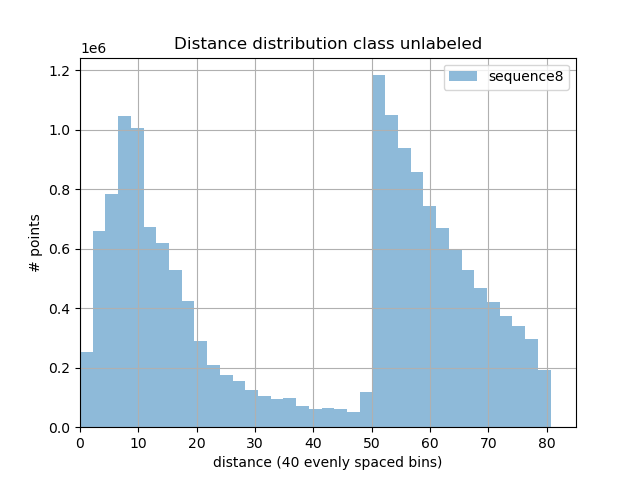
\includegraphics[width=\textwidth]{Figures/Chapter4/dist-height/dist/test/class0.png}
     \end{subfigure}
     \hfill
     \begin{subfigure}[b]{0.24\textwidth}
         \centering
         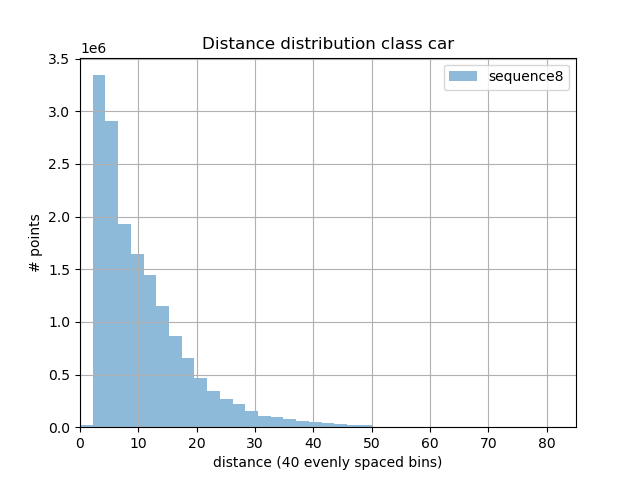
\includegraphics[width=\textwidth]{Figures/Chapter4/dist-height/dist/test/class1.png}
     \end{subfigure}
     \begin{subfigure}[b]{0.24\textwidth}
         \centering
         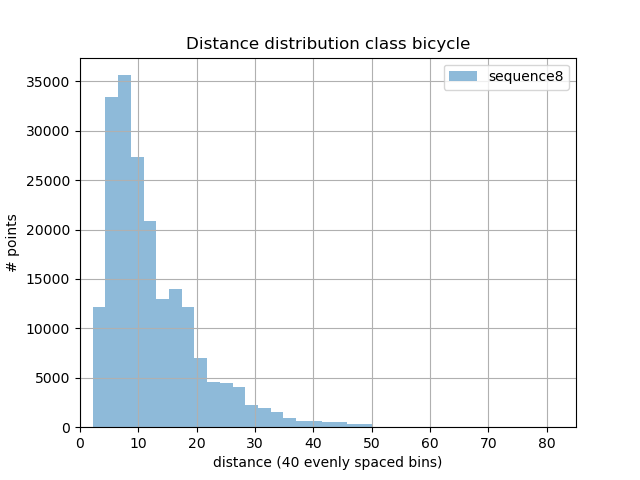
\includegraphics[width=\textwidth]{Figures/Chapter4/dist-height/dist/test/class2.png}
     \end{subfigure}
     \hfill
     \begin{subfigure}[b]{0.24\textwidth}
         \centering
         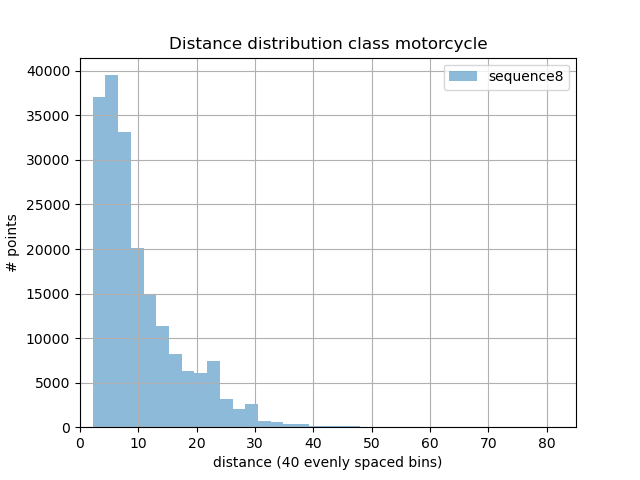
\includegraphics[width=\textwidth]{Figures/Chapter4/dist-height/dist/test/class3.png}
     \end{subfigure}
     \begin{subfigure}[b]{0.24\textwidth}
         \centering
         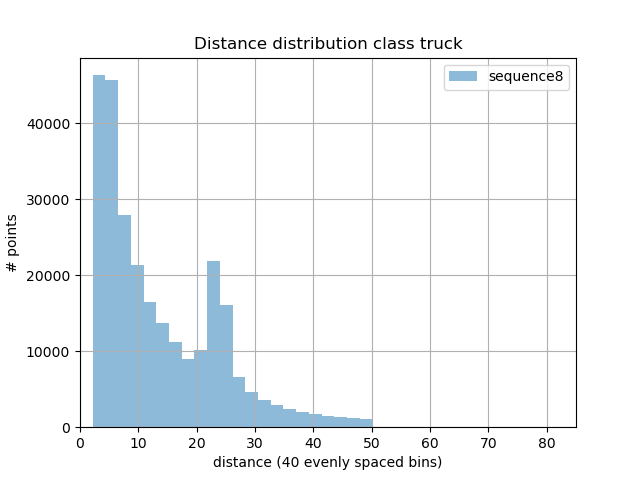
\includegraphics[width=\textwidth]{Figures/Chapter4/dist-height/dist/test/class4.png}
     \end{subfigure}
     \hfill
     \begin{subfigure}[b]{0.24\textwidth}
         \centering
         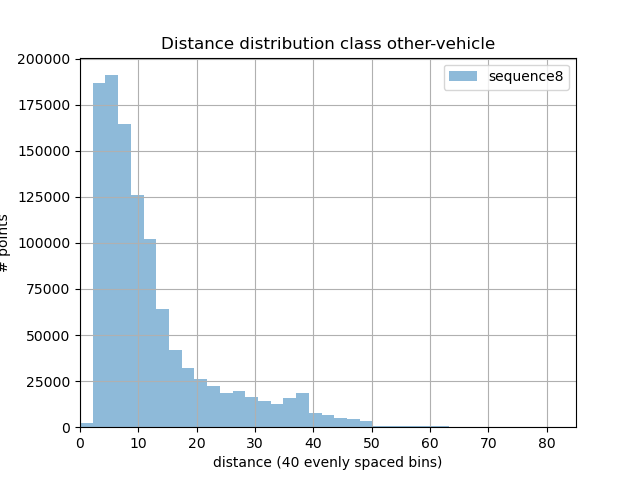
\includegraphics[width=\textwidth]{Figures/Chapter4/dist-height/dist/test/class5.png}
     \end{subfigure}
     \begin{subfigure}[b]{0.24\textwidth}
         \centering
         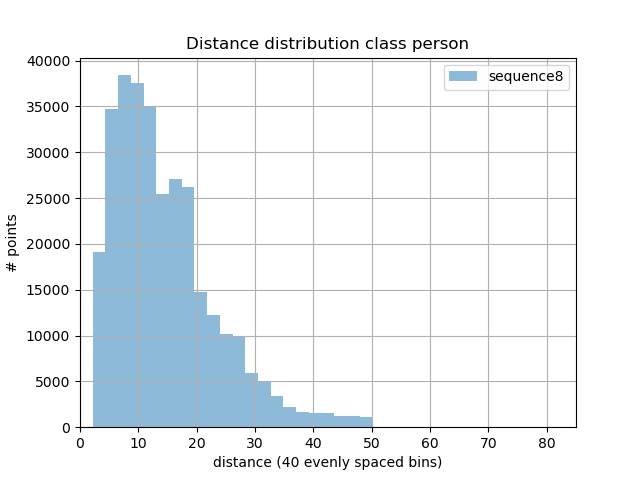
\includegraphics[width=\textwidth]{Figures/Chapter4/dist-height/dist/test/class6.png}
     \end{subfigure}
     \hfill
     \begin{subfigure}[b]{0.24\textwidth}
         \centering
         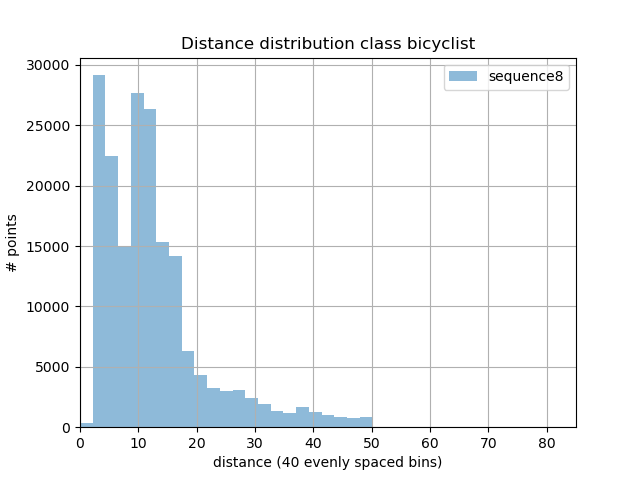
\includegraphics[width=\textwidth]{Figures/Chapter4/dist-height/dist/test/class7.png}
     \end{subfigure}
     \begin{subfigure}[b]{0.24\textwidth}
         \centering
         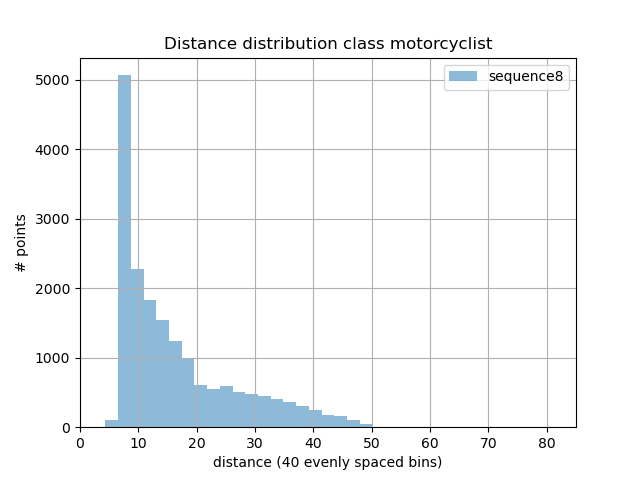
\includegraphics[width=\textwidth]{Figures/Chapter4/dist-height/dist/test/class8.png}
     \end{subfigure}
     \hfill
     \begin{subfigure}[b]{0.24\textwidth}
         \centering
         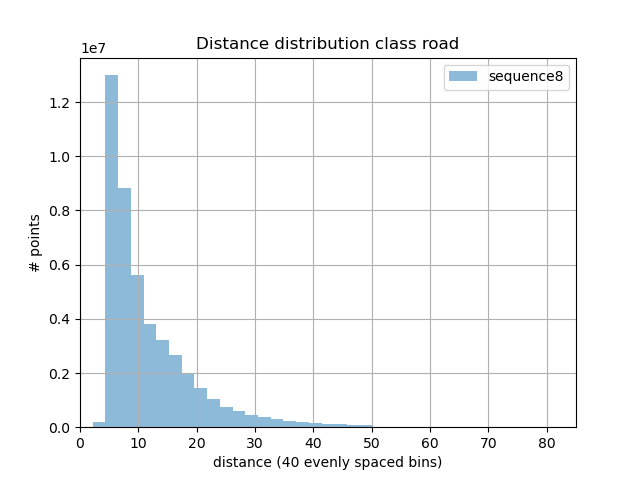
\includegraphics[width=\textwidth]{Figures/Chapter4/dist-height/dist/test/class9.png}
     \end{subfigure}
     \begin{subfigure}[b]{0.24\textwidth}
         \centering
         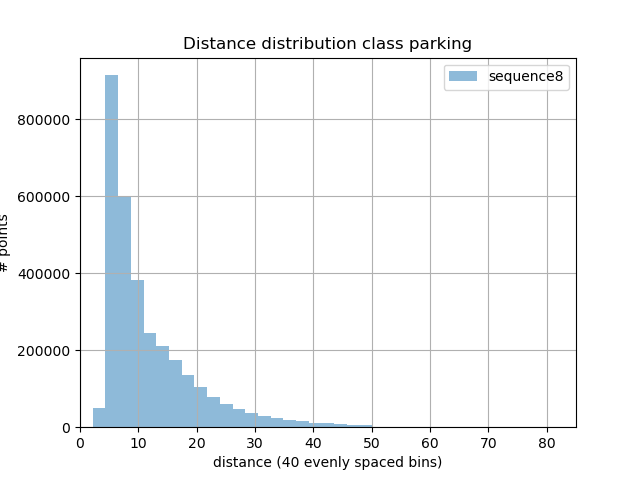
\includegraphics[width=\textwidth]{Figures/Chapter4/dist-height/dist/test/class10.png}
     \end{subfigure}
     \hfill
     \begin{subfigure}[b]{0.24\textwidth}
         \centering
         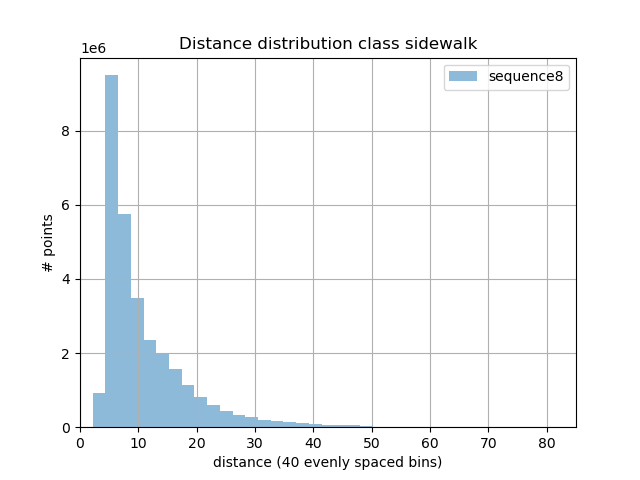
\includegraphics[width=\textwidth]{Figures/Chapter4/dist-height/dist/test/class11.png}
     \end{subfigure}
     \begin{subfigure}[b]{0.24\textwidth}
         \centering
         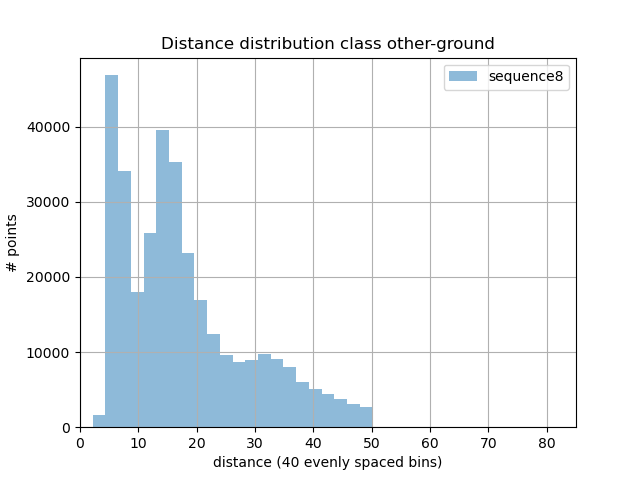
\includegraphics[width=\textwidth]{Figures/Chapter4/dist-height/dist/test/class12.png}
     \end{subfigure}
     \hfill
     \begin{subfigure}[b]{0.24\textwidth}
         \centering
         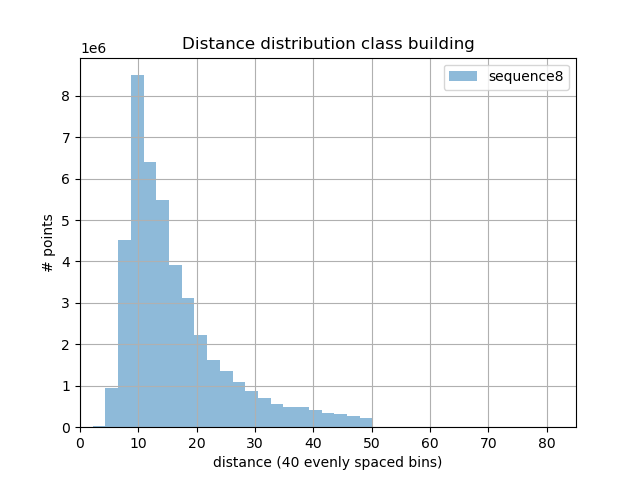
\includegraphics[width=\textwidth]{Figures/Chapter4/dist-height/dist/test/class13.png}
     \end{subfigure}
     \begin{subfigure}[b]{0.24\textwidth}
         \centering
         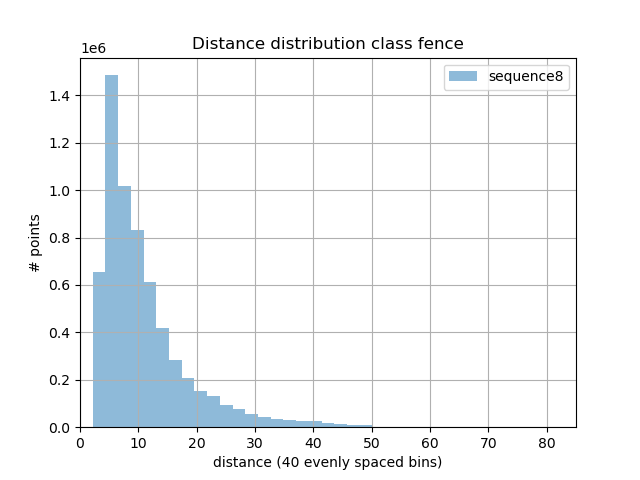
\includegraphics[width=\textwidth]{Figures/Chapter4/dist-height/dist/test/class14.png}
     \end{subfigure}
     \hfill
     \begin{subfigure}[b]{0.24\textwidth}
         \centering
         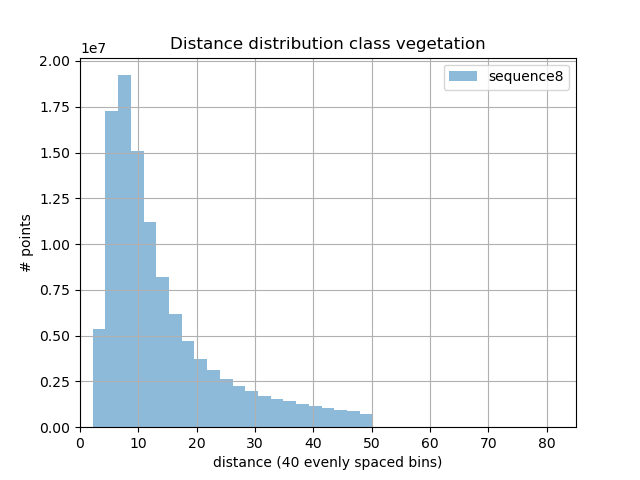
\includegraphics[width=\textwidth]{Figures/Chapter4/dist-height/dist/test/class15.png}
     \end{subfigure}
     \begin{subfigure}[b]{0.24\textwidth}
         \centering
         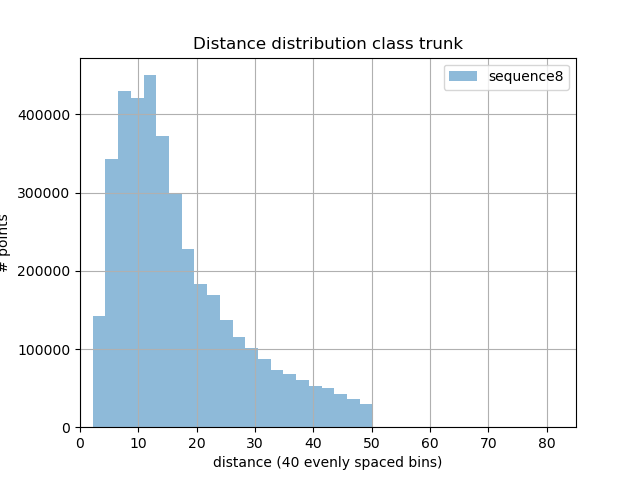
\includegraphics[width=\textwidth]{Figures/Chapter4/dist-height/dist/test/class16.png}
     \end{subfigure}
     \hfill
     \begin{subfigure}[b]{0.24\textwidth}
         \centering
         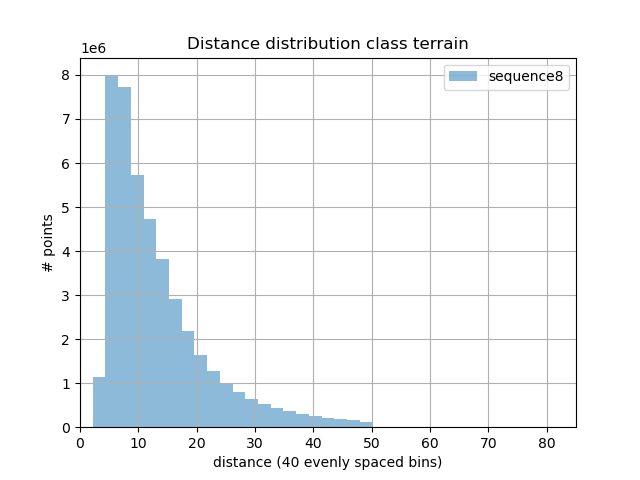
\includegraphics[width=\textwidth]{Figures/Chapter4/dist-height/dist/test/class17.png}
     \end{subfigure}
     \begin{subfigure}[b]{0.24\textwidth}
         \centering
         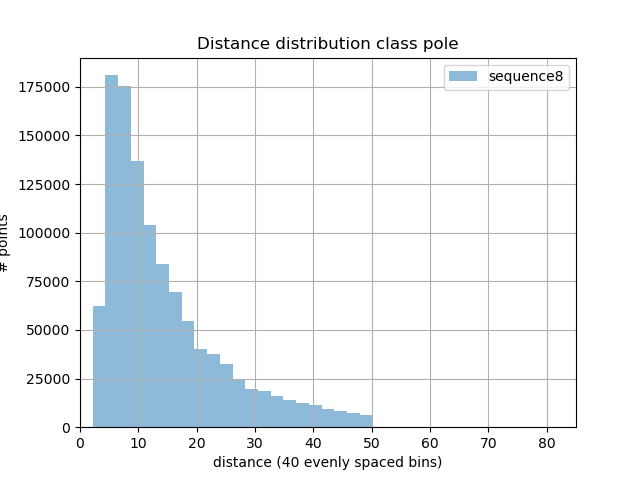
\includegraphics[width=\textwidth]{Figures/Chapter4/dist-height/dist/test/class18.png}
     \end{subfigure}
     \hfill
     \begin{subfigure}[b]{0.24\textwidth}
         \centering
         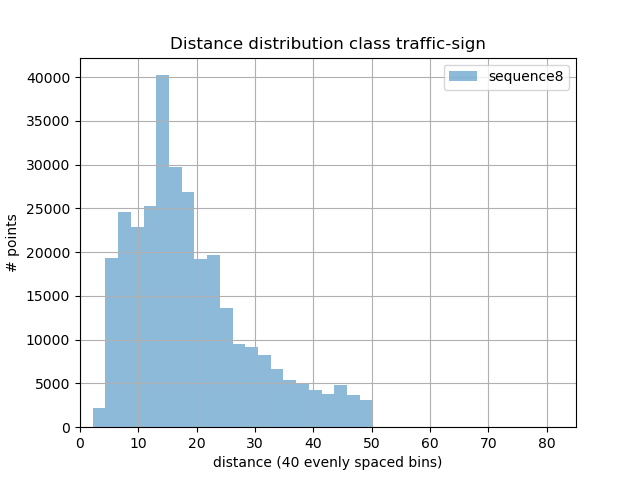
\includegraphics[width=\textwidth]{Figures/Chapter4/dist-height/dist/test/class19.png}
     \end{subfigure}
\caption{Example compuond figure.}        
\label{fig:distances}
\end{figure}
\end{appendices}
\chapter*{Acknowledgements}\label{ch:ack}
Lorem ipsum dolor sit amet, consectetur adipisci elit, sed eiusmod tempor incidunt ut labore et dolore magna aliqua. Ut enim ad minim veniam, quis nostrum exercitationem ullam corporis suscipit laboriosam, nisi ut aliquid ex ea commodi consequatur. Quis aute iure reprehenderit in voluptate velit esse cillum dolore eu fugiat nulla pariatur. Excepteur sint obcaecat cupiditat non proident, sunt in culpa qui officia deserunt mollit anim id est laborum.

%%%%%%%%%%%%  BIBLIOGRAPHY  %%%%%%%%%%%%%%%%%
%\bibliographystyle{plain} % We choose the "plain" reference style
\bibliography{bibliography} % Entries are in the "refs.bib" file

\end{document}

\endinput


%%% Local Variables: 
%%% mode: latex
%%% TeX-master: t
%%% TeX-source-specials-mode: t
%%% TeX-PDF-mode: t
%%% End: 
